\centering
\section*{\myul{Physikalische Eigenschaften}}

\begin{tikzpicture}[remember picture, overlay]

% --- ERSTE REIHE: Am Seitenursprung anfangen
\setlength{\rowheight}{50mm}

    % A1) Erste Kachel relativ zum Seitenursprung
    \setlength{\cellwidth}{55mm}
    \Tile{A1}{([xshift=10mm, yshift=-18mm]current page.north west)}{\cellwidth}{\rowheight}
        {
            \vspace{-\TileSep}
            \titlerm{Knudsen-Zahl}\\ \vspace{-3mm}
            \begin{equation*}
                \mathrm{Kn} = \frac{\bar{\lambda}}{L}
            \end{equation*}
            {\scriptsize
            \vspace{-3mm}
            \begin{align*}
                \bar{\lambda} &= \text{Mittlere freie Weglänge} \\
                L             &= \text{Charakteristische Länge}
            \end{align*}%
            \vspace{-7mm}
            \begin{align*}
                \text{Kontinuumsströmung: }    \mathrm{Kn} &< 10^{-2} \\
                \text{Freie Molekülströmung: } \mathrm{Kn} &> 10
            \end{align*}%
            \vspace{-5mm}
            \begin{tabular}{c|r|r|r}
                \xrowht[()]{1.6mm} Höhe            & 0\,km         &  80\,km &  150\,km \\ \hline
                \xrowht[()]{1.6mm} $\bar{\lambda}$ & 3\,nm         & 100\,nm & 2000\,nm \\ \hline
                \xrowht[()]{1.6mm} L               & 1,6\,$\upmu$m &   3\,cm &  200\,m
            \end{tabular}
            }
        }{0}{1}{1}{0}

    % B1) Zweite Kachel rechts anbauen
    \setlength{\cellwidth}{55mm}
    \Tile{B1}{(A1.north east)}{\cellwidth}{\rowheight}
        {
            \vspace{-\TileSep}
            \titlerm{Dichte}\vspace{-0.5mm}
            \begin{align*}
                \text{Flüssigkeiten: }    \rho &= \text{konst.} \\
                \text{Barotrope Fluide: } \rho &= \rho\!\left(p\right) \\
                \text{Gase: }             \rho &= \rho\!\left(p, T\right)
            \end{align*}%
            \vspace{-6mm}
            \rule{\dimexpr\cellwidth-2\TileSep}{0.5pt} \\ \vspace{1mm}
            \titlerm{Druck}\vspace{-0.5mm}
            \begin{equation*}
                p_\text{ges} = p_\text{stat} + p_\text{dyn}
            \end{equation*}
            \begin{equation*}
                p_\text{dyn} = q = \frac{1}{2}\,\rho\,v^2
            \end{equation*}
        }{0}{1}{1}{0}

    % C1) Dritte Kachel rechts anbauen
    \setlength{\cellwidth}{80mm}
    \Tile{C1}{(B1.north east)}{\cellwidth}{\rowheight}
        {
            \vspace{-\TileSep}
            \titlerm{Ideale Gasgleichung}\vspace{1mm}
            \begin{minipage}{0.4\cellwidth-\TileSep}
                \centering
                \vspace{-3mm}
                \begin{equation*}
                    p = \rho\,R\,T
                \end{equation*}
                \vspace{-4mm}
            \end{minipage}%
            \vline
            \begin{minipage}{0.4\cellwidth-\TileSep}
                \centering
                \vspace{-3mm}
                \begin{equation*}
                    p\,V = m\,R\,T
                \end{equation*}
                \vspace{-4mm}
            \end{minipage}%
            \vspace{0.1mm}
            \rule{\dimexpr\cellwidth-2\TileSep}{0.5pt} \\ \vspace{1mm}
            \titlerm{Spezifische Gaskonstante}\\ \vspace{-4mm}
            \begin{equation*}
                R = \frac{\Re}{M} = c_\text{p} - c_\text{v}
            \end{equation*}
            {\scriptsize
            \vspace{-4mm}
            \begin{align*}
                \Re &= \text{8314,3}\,\tfrac{\text{J}}{\text{kmol}\,\text{K}} \\
                M   &= \text{Molare Masse} \\
                c_p &= \text{Spezifische Wärme bei konstantem Druck} \\
                c_v &= \text{Spezifische Wärme bei konstanter Temperatur}
            \end{align*}
            }
        }{0}{0}{1}{0}

% --- ZWEITE REIHE: Unten anbauen
\setlength{\rowheight}{55mm}

    % A2) Erste Kachel unten anbauen
    \setlength{\cellwidth}{115mm}
    \Tile{A2}{(A1.south west)}{\cellwidth}{\rowheight}
        {
            \titlerm{Polytrope Zustandsänderung}\\ \vspace{2mm}
            \begin{minipage}{0.55\cellwidth-\TileSep}
                \centering
                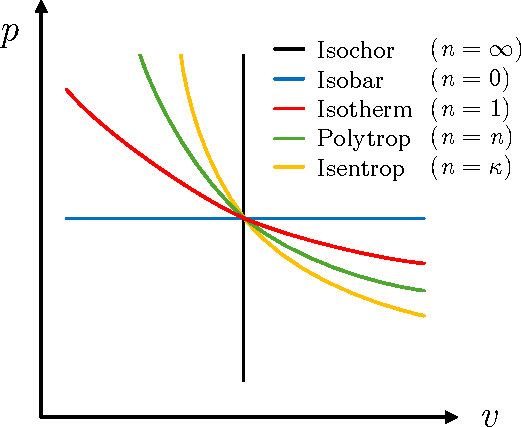
\includegraphics[width=52mm]{images/polytropen.pdf}
            \end{minipage}%
            \begin{minipage}{0.45\cellwidth-\TileSep}
                \centering
                \begin{equation*}
                    \frac{p}{\rho^n} = n\,v^n = \text{konst.}
                \end{equation*}%
                \vspace{-3.5mm}
                \begin{equation*}
                    \frac{\rho}{\rho_\text{b}} = \left(\frac{p}{p_\text{b}}\right)^{\frac{1}{n}}
                \end{equation*}%
                \vspace{-2.5mm}
                \begin{align*}
                         n &= \text{Polytropenexponent} \\
                    \kappa &= \text{Isentropenexponent}
                \end{align*}
                \begin{equation*}
                    \kappa = \frac{c_p}{c_v} = \frac{c_p}{c_p - R} = \frac{c_v + R}{c_v}
                \end{equation*}
            \end{minipage}
        }{0}{1}{1}{0}

    % B2) Zweite Kachel rechts anbauen
    \setlength{\cellwidth}{75mm}
    \Tile{B2}{(A2.north east)}{\cellwidth}{\rowheight}
        {
            \titlerm{Schallgeschwindigkeit}\\ \vspace{-2.5mm}
            \begin{align*}
                c &= \sqrt{\left(\frac{\partial p}{\partial\rho}\right)_s} = \sqrt{\kappa\left(\frac{\partial p}{\partial\rho}\right)_T} \\
                  &= \underbrace{\sqrt{\kappa\,R\,T} = \sqrt{\kappa\,\frac{p}{\rho}}}_\text{Ideales Gas}
            \end{align*}%
            \vspace{1mm}
            \begin{equation*}
                \underbrace{\frac{\Delta\rho}{\rho} \approx \frac{\mathrm{Ma}^2}{2}}_\text{Grenze Inkompressibler Strömung}
            \end{equation*}
        }{0}{0}{1}{0}

% --- DRITTE REIHE: Unten anbauen
\setlength{\rowheight}{39mm}

    % A3) Erste Kachel unten anbauen
    \setlength{\cellwidth}{60mm}
    \Tile{A3}{(A2.south west)}{\cellwidth}{\rowheight}
        {
            \titlerm{Temperatur}\\ \vspace{-2mm}
            \begin{equation*}
                E_\text{kin} = \frac{3}{2}\,k_\text{B}\,T
            \end{equation*}
            {\scriptsize
            \vspace{-3mm}
            \begin{align*}
                E_\text{kin} &= \text{kinetische Energie} \\[0.5ex]
                k_\text{B}   &= \text{Boltzmann-Konstante} \\[-0.5ex]
                             &= \text{1,38}\cdot 10^{-23}\,\tfrac{\text{J}}{\text{K}} \\[0.5ex]
                T            &= \text{Temperatur}
            \end{align*}
            }
        }{0}{1}{1}{0}

    % B3) Zweite Kachel rechts anbauen
    \setlength{\cellwidth}{65mm}
    \Tile{B3}{(A3.north east)}{\cellwidth}{\rowheight}
        {
            \titlerm{Newton'sches Reibungsgesetz}\\ \vspace{-2mm}
            \begin{equation*}
                \tau = \eta\,\frac{\text{d}u}{\text{d}y} = \eta\,D
            \end{equation*}
            {\scriptsize
            \vspace{-3mm}
            \begin{align*}
                \tau &= \text{Schubspannung} \\
                \eta &= \text{Dynamische Viskosität }\left[\tfrac{\text{kg}}{\text{m}\,\text{s}}\right] \\
                D    &= \text{Schergeschwindigkeit}
            \end{align*}
            }
        }{0}{1}{1}{0}

    % C3) Dritte Kachel rechts anbauen
    \setlength{\cellwidth}{65mm}
    \Tile{C3}{(B3.north east)}{\cellwidth}{\rowheight}
        {
            \titlerm{Kinematische Viskosität}\\ \vspace{-2mm}
            \begin{equation*}
                \nu = \frac{\eta}{\rho}
            \end{equation*}
            {\scriptsize
            \vspace{-2.5mm}
            \begin{align*}
                \nu  &= \text{Kinematische Viskosität }\left[\tfrac{\text{m}^2}{\text{s}}\right] \\
                \eta &= \text{Dynamische Viskosität }\left[\tfrac{\text{kg}}{\text{m}\,\text{s}}\right] \\
                \rho &= \text{Dichte}
            \end{align*}
            }
        }{0}{0}{1}{0}

\end{tikzpicture}